%
% $Id$
%

\documentclass[letter,landscape]{seminar}

\usepackage{pstcol}
\usepackage{slidesec}
\usepackage{semcolor}

\input{seminar.bug}
\input{seminar.bg2}

\usepackage{graphics}
\usepackage{fancybox}
\usepackage{fancyhdr}
\usepackage{epsfig}

% Headers and footers personalization using the `fancyhdr' package
\fancyhf{} % Clear all fields
\renewcommand{\headrulewidth}{0.2mm}
\renewcommand{\footrulewidth}{0.2mm}
\fancyhead[C]{\Large\textbf{SLURM Design - The Big Picture}}
%\fancyfoot[L]{\tiny\thedate}
\fancyfoot[L]{
\includegraphics[scale=0.075]{penguin.eps}\\\tiny LINUX} 
%\fancyfoot[R]{\small LLNL}
\fancyfoot[R]{
\includegraphics[scale=0.2]{llnl.ps}\\\tiny LLNL} 
\fancyfoot[C]{\tiny Page \theslide}

% Create room for headers and footers
\renewcommand{\slidetopmargin}{2cm}
\renewcommand{\slidebottommargin}{3cm}

% Center horizontally the headers and footers (see seminar.bug)
\renewcommand{\headwidth}{\textwidth}

% To adjust the frame length to the header and footer ones
\autoslidemarginstrue

% Hook to tell dvips to print in landscape mode
\def\printlandscape{\special{landscape}}

% Possibilities: shadow, oval, double, none, plain
\slideframe{none}

% display grey text diagonally across background of each slide
%\definecolor{LightGray}{gray}{0.85}
%\newslideframe{BackgroundText}{%
%  \boxput{\rotatebox{56}{\scalebox{4.5}{%
%    \textcolor{LightGray}{CONFIDENTIAL}}}}{#1}}
%\slideframe*{BackgroundText}

% Put an image in the background of each slide
%\newslideframe{IMAGE}{%
%  \boxput{\rput(1,0){\includegraphics[scale=1.0]{kaos_logo2.ps}}}{#1}}
%\slideframe*{IMAGE}

% This allows text to be blued with \textcolor{Blue}{my text}
\definecolor{Blue}{rgb}{0.,0.,1.}
\definecolor{Gold}{rgb}{1.,0.84,0.}
\definecolor{Pink}{rgb}{1.,0.75,0.8}

\begin{document}

\slidepagestyle{fancy}

% The presentation begins here.

\begin{slide}
  %\slideheading{The Big Picture}
\begin{center}

\epsfig{file=slurm.eps,scale=0.50}
\end{center}
\end{slide}


\begin{slide}
  \slideheading{General Characteristics}
  \begin{itemize}
    \item{Simplicity}
    \item{Open Source - GPL}
    \item{Portable - C, autoconf}
    \item{Interconnect independence - IP, QSW, open ended}
    \item{Scalability - $2^{16}$}
    \item{Fault Tolerance}
    \item{Secure - K5/DCE, ???}
    \item{Sys admin friendly}
  \end{itemize}
\end{slide}

\begin{slide}
  \slideheading{What is SLURM?}
  \begin{itemize}
    \item{Functions: allocate, execute, arbitrate}
    \item{Users: {\tt srun}, {\tt scancel}, {\tt squeue}}
    \item{Admins: {\tt slurmadmin}}
    \item{API for external metabatch systems and schedulers}
    \item{Daemons: {\tt slurmd} on compute nodes, {\tt slurmctld} on management node}
  \end{itemize}
\end{slide}

\begin{slide}
  \slideheading{What is !SLURM?}
  \begin{itemize}
    \item{Not a sophisticated batch scheduler}
    \item{Not a Gang scheduler - no time sharing}
    \item{Not a Metabatch system - one cluster only}
    \item{Not a comprehensive monitoring/cluster admin tool}
  \end{itemize}
\end{slide}


\begin{slide}
  \slideheading{Architecture}
\begin{center}
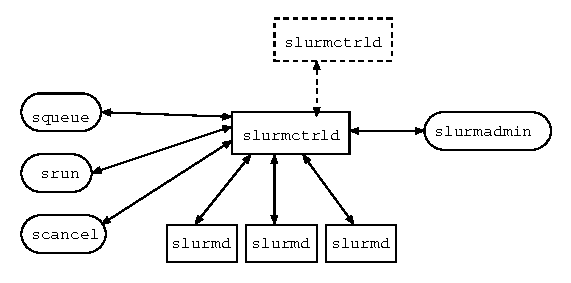
\epsfig{file=arch.eps,scale=0.80}
\end{center}
\end{slide}


\begin{slide}
  \slideheading{Slurmd}
  \begin{itemize}
    \item{Machine and Job Status Service}
    \item{Process Manager}
    \item{Stream Copy Service}
  \end{itemize}
\end{slide}

\begin{slide}
  \slideheading{Controller}
  \begin{itemize}
    \item{Machine Status Manager}
    \item{Partition Manager}
    \item{Scheduler}
    \item{Job Manager}
    \item{Job Status Manager}
    \item{Switch Manager}
  \end{itemize}
\end{slide}

\begin{slide}
  \slideheading{Command Line Utilities}
  \begin{itemize}
    \item{{\tt srun}: submit job}
    \item{{\tt squeue}: list queue of running/waiting jobs}
    \item{{\tt scancel}: cancel running/waiting job}
    \item{{\tt slurmadmin}: root only privileged commands}
  \end{itemize}
\end{slide}


\begin{slide}
  \slideheading{Communications Layer}
  \begin{center}?
  \end{center}
\end{slide}

\begin{slide}
  %\slideheading{Example: batch job}
  {\tt \$ srun --batch --nodes=2 --nprocs=2 mping 1 1048576}\\
  {\tt srun: pbatch-42}\\
  {\tt \$}
  \begin{itemize}
    \item{{\tt srun} authenticates, submits request to controller}
    \item{Will job ever run?  Immediate error if not.}
    \item{Assign batch ID, enqueue}
    \item{Scheduler reorders queue}
    \item{Job manager scan for cleanup}
    \item{Job manager scan for startup}
    \item{Allocate nodes from partition manager}
    \item{Send request to {\tt slurmd}'s on allocated nodes}
    \item{Begin job status monitoring}
    \item{When complete, trigger job manager cleanup}
  \end{itemize}
\end{slide}

\begin{slide}
  \slideheading{Stdin/Stdout/Stderr}
  \begin{itemize}
    \item{Copy stdin to file on compute node(s) before starting}
    \item{Spool stdout/stderr to files on compute node}
    \item{Controller copies and merges when job complete}
    \item{Interactive {\tt srun} ``tails'' files directly from {\tt slurmd}'s}
  \end{itemize}
\end{slide}

\begin{slide}
  %\slideheading{Example: batch job}
  {\tt \$ srun --nodes=2 --nprocs=2 mping 1 1048576}\\
  {\tt srun: pbatch-42}\\
  {\tt 1 pinged   0:        1 bytes      5.38 uSec     0.19 MB/s}\\
  {\tt 1 pinged   0:        2 bytes      5.32 uSec     0.38 MB/s}\\
  {\tt ...}\\
  {\tt \$}
  Same sequence as batch except:
  \begin{itemize}
    \item{{\tt srun} doesn't go away after job is started}
    \item{Controller sends list of hosts and {\em nonce}}
    \item{{\tt srun} connects to {\tt slurmd}'s and tails stdout/stderr}
    \item{{\tt srun} gets EOF on stdout/stderr streams on termination}
    \item{Or Control-C sends abort message to {\tt slurmd's} and 
          controller cleans up}
    \item{Way to detach {\tt srun} from job and let it continue as batch}
  \end{itemize}
\end{slide}


\end{document}
